\chapter{Azure DevOps}


\section{About Azure DevOps Enterprise \& Cloud}

Azure DevOps Enterprise is an on-premise variation of the cloud-hosted Azure DevOps services.
Both versions are compatible with \cxoneflow and are generically referred to Azure DevOps Enterprise
throughout this documentation.

\noindent\\The \cxoneflow endpoint \texttt{/adoe} is the handler for all webhook event
payloads originating from Azure DevOps Enterprise.  

\section{Webhook Configuration}

Azure DevOps Enterprise organizes source repositories at the top level by a \textit{Collection};
at least one collection will exist and many organizations will keep the installation-default
collection named \texttt{DefaultCollection}.  In each collection will exist one or more
\textit{Projects} and in each project will exist one or more \textit{Repositories}.  
Webhook configurations can be applied to a single repository via the repository configuration.
Applying the configuration at the level of each individual repository is usually suitable
for testing purposes only.

Webhook configurations applied at the \textit{Project} level can be configured to invoke webhook
events for all repositories in the project.  This is the most ideal location to configure
the webhook endpoints.  The project name will appear in clone URLs and can be used as part of 
the regular expression placed in the \texttt{repo-match} configuration element.  Please see 
Section \ref{sec:scm-block-element} for a description of the \texttt{repo-match} configuration
element.

The project's "Service Hooks" can be used to configure webhook events to be delivered to the
\cxoneflow \texttt{/adoe} endpoint for each repository in the organization.  Azure DevOps
Enterprise will require multiple service hook definitions to handle different classes
of repository events.

Figure \ref{fig:adoe-hook-config} shows the initial service hook configuration with the 
"Web Hooks" option selected.  Clicking the \textbf{Next} button will display the 
event trigger configuration as depicted in Figure \ref{fig:adoe-trigger-config}. 
The trigger type of event for \textbf{Code pushed} should be selected.
Clicking the \textbf{Next} button will display the \textbf{Action} configuration
where the webhook connection parameters can be configured.

Figure \ref{fig:adoe-endpoint-config} shows the configuration where the \cxoneflow
endpoint connection configuration is to be provided.  A URL with the suffix
\texttt{/adoe} and the \textit{Basic authentication password} are the only
fields that are required by \cxoneflow\footnote{Azure DevOps Enterprise will require
the use of an encrypted endpoint when using the basic authorization password.}.
The basic authentication password should match the \texttt{shared-secret} \cxoneflow
configuration element.  Please see section \ref{sec:connection-element}
for more information about the \texttt{shared-secret} configuration.

The \textbf{Test} button can be used to validate connectivity to the \cxoneflow endpoint.
The secret is not currently part of the connectivity validation; if the \cxoneflow logs
are showing messages indicating webhook events are being rejected, checking that the
shared secret matches in both the Azure DevOps Enterprise service hook and \cxoneflow
configurations.

A complete configuration should emit web hook payloads on the following events:

\begin{itemize}
    \item Code pushed
    \item Pull request created
    \item Pull request updated
\end{itemize}

\begin{figure}[ht]
    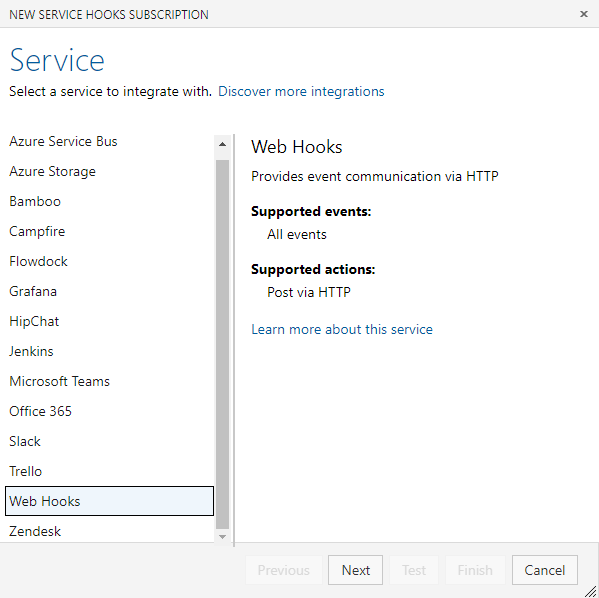
\includegraphics[width=\textwidth]{graphics/adoe-service-hooks-sub.png}
    \caption{Azure DevOps Enterprise Service Hook Configuration}
    \label{fig:adoe-hook-config}
\end{figure}

\begin{figure}[ht]
    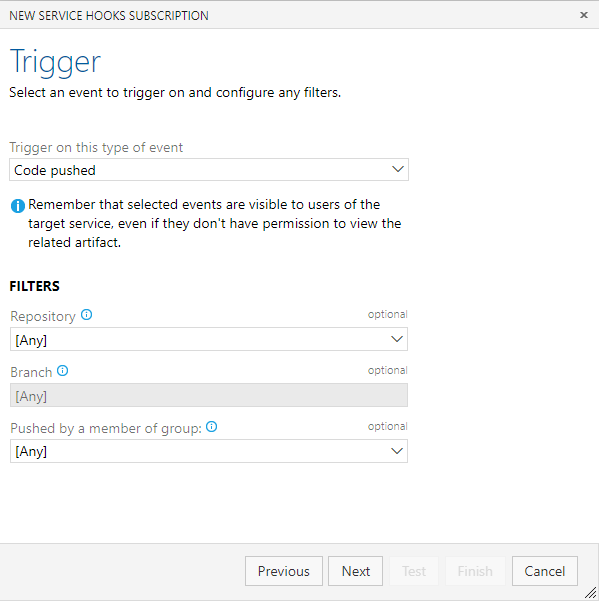
\includegraphics[width=\textwidth]{graphics/adoe-hook-trigger-config.png}
    \caption{Azure DevOps Enterprise Web Hook Trigger Configuration}
    \label{fig:adoe-trigger-config}
\end{figure}

\begin{figure}[ht]
    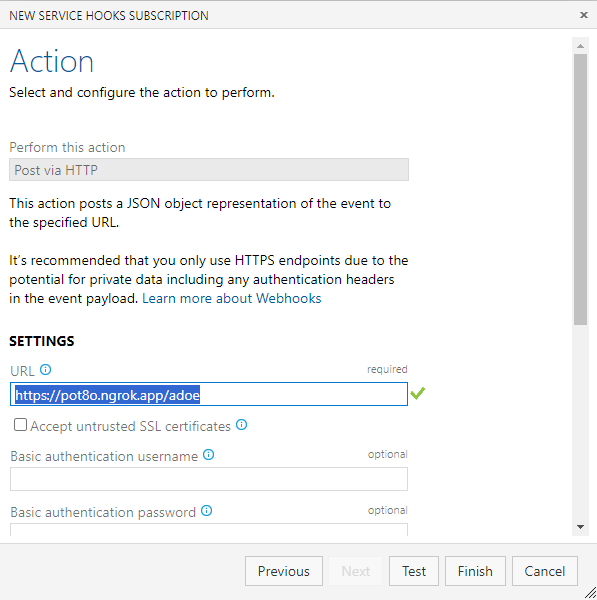
\includegraphics[width=\textwidth]{graphics/adoe-hook-endpoint-config.png}
    \caption{Azure DevOps Enterprise Web Hook Endpoint Configuration}
    \label{fig:adoe-endpoint-config}
\end{figure}

\section{\cxoneflow Service Account}

Azure DevOps Enterprise utilizes user accounts to define access.  \cxoneflow will require
at least one user account to use as a service account for API and cloning operations.  The
service account must be in the \textit{Contributor} group for each project for which
that account will orchestrate scans.  It is possible to create a single service account that
is used for all projects if the service account is assigned as a contributor to all
relevant projects.  The \cxoneflow configuration can accommodate multiple user accounts
if there is a need to have separate service accounts for some projects.

\section{\cxoneflow SSH Keys}

While performing scan orchestration, \cxoneflow does access the Azure DevOps Enterprise API for
certain operations.  This requires a configuration in the \texttt{api-auth} configuration
element as described in Section \ref{sec:api-auth-element}.  The \texttt{clone-auth},
described in Section \ref{sec:clone-auth-element}, is an optional element where the credentials
used for cloning code can be provided.  If \texttt{clone-auth} is not provided, cloning will
be attempted using the credentials defined by \texttt{api-auth}.

The \texttt{clone-auth} configuration can define an SSH private key for use in cloning.  This
will allow for a separate set of credentials or authentication methods between cloning and
API use.

\section{Protected Branches}

Each repository in Azure DevOps Enterprise has a default branch defined in the project
configuration.  The repository's default branch is considered the protected branch for
workflow logic purposes.